\chapter{Appendix}\label{sec:chapAppendix}
\setheader{Appendix}

\section{Contact Information and Code Access}
If you have any questions regarding this work, feel free to contact me at j.francisco.ribera@gmail.com. Given that the Melkroboter proyect is looking to request Patent rights, the code might not be available for public access.
% \section{Other Algorithm Evaluations}
%     \begin{itemize}
%         \item DOPE performance
%     \end{itemize}
% \section{Official Assignment}
% TODO: copy paste from moodle

\newpage
\section{Synthetic Dataset Generation Overview}
\label{appendix:ndds}

\begin{figure}[!ht]
    \centering
    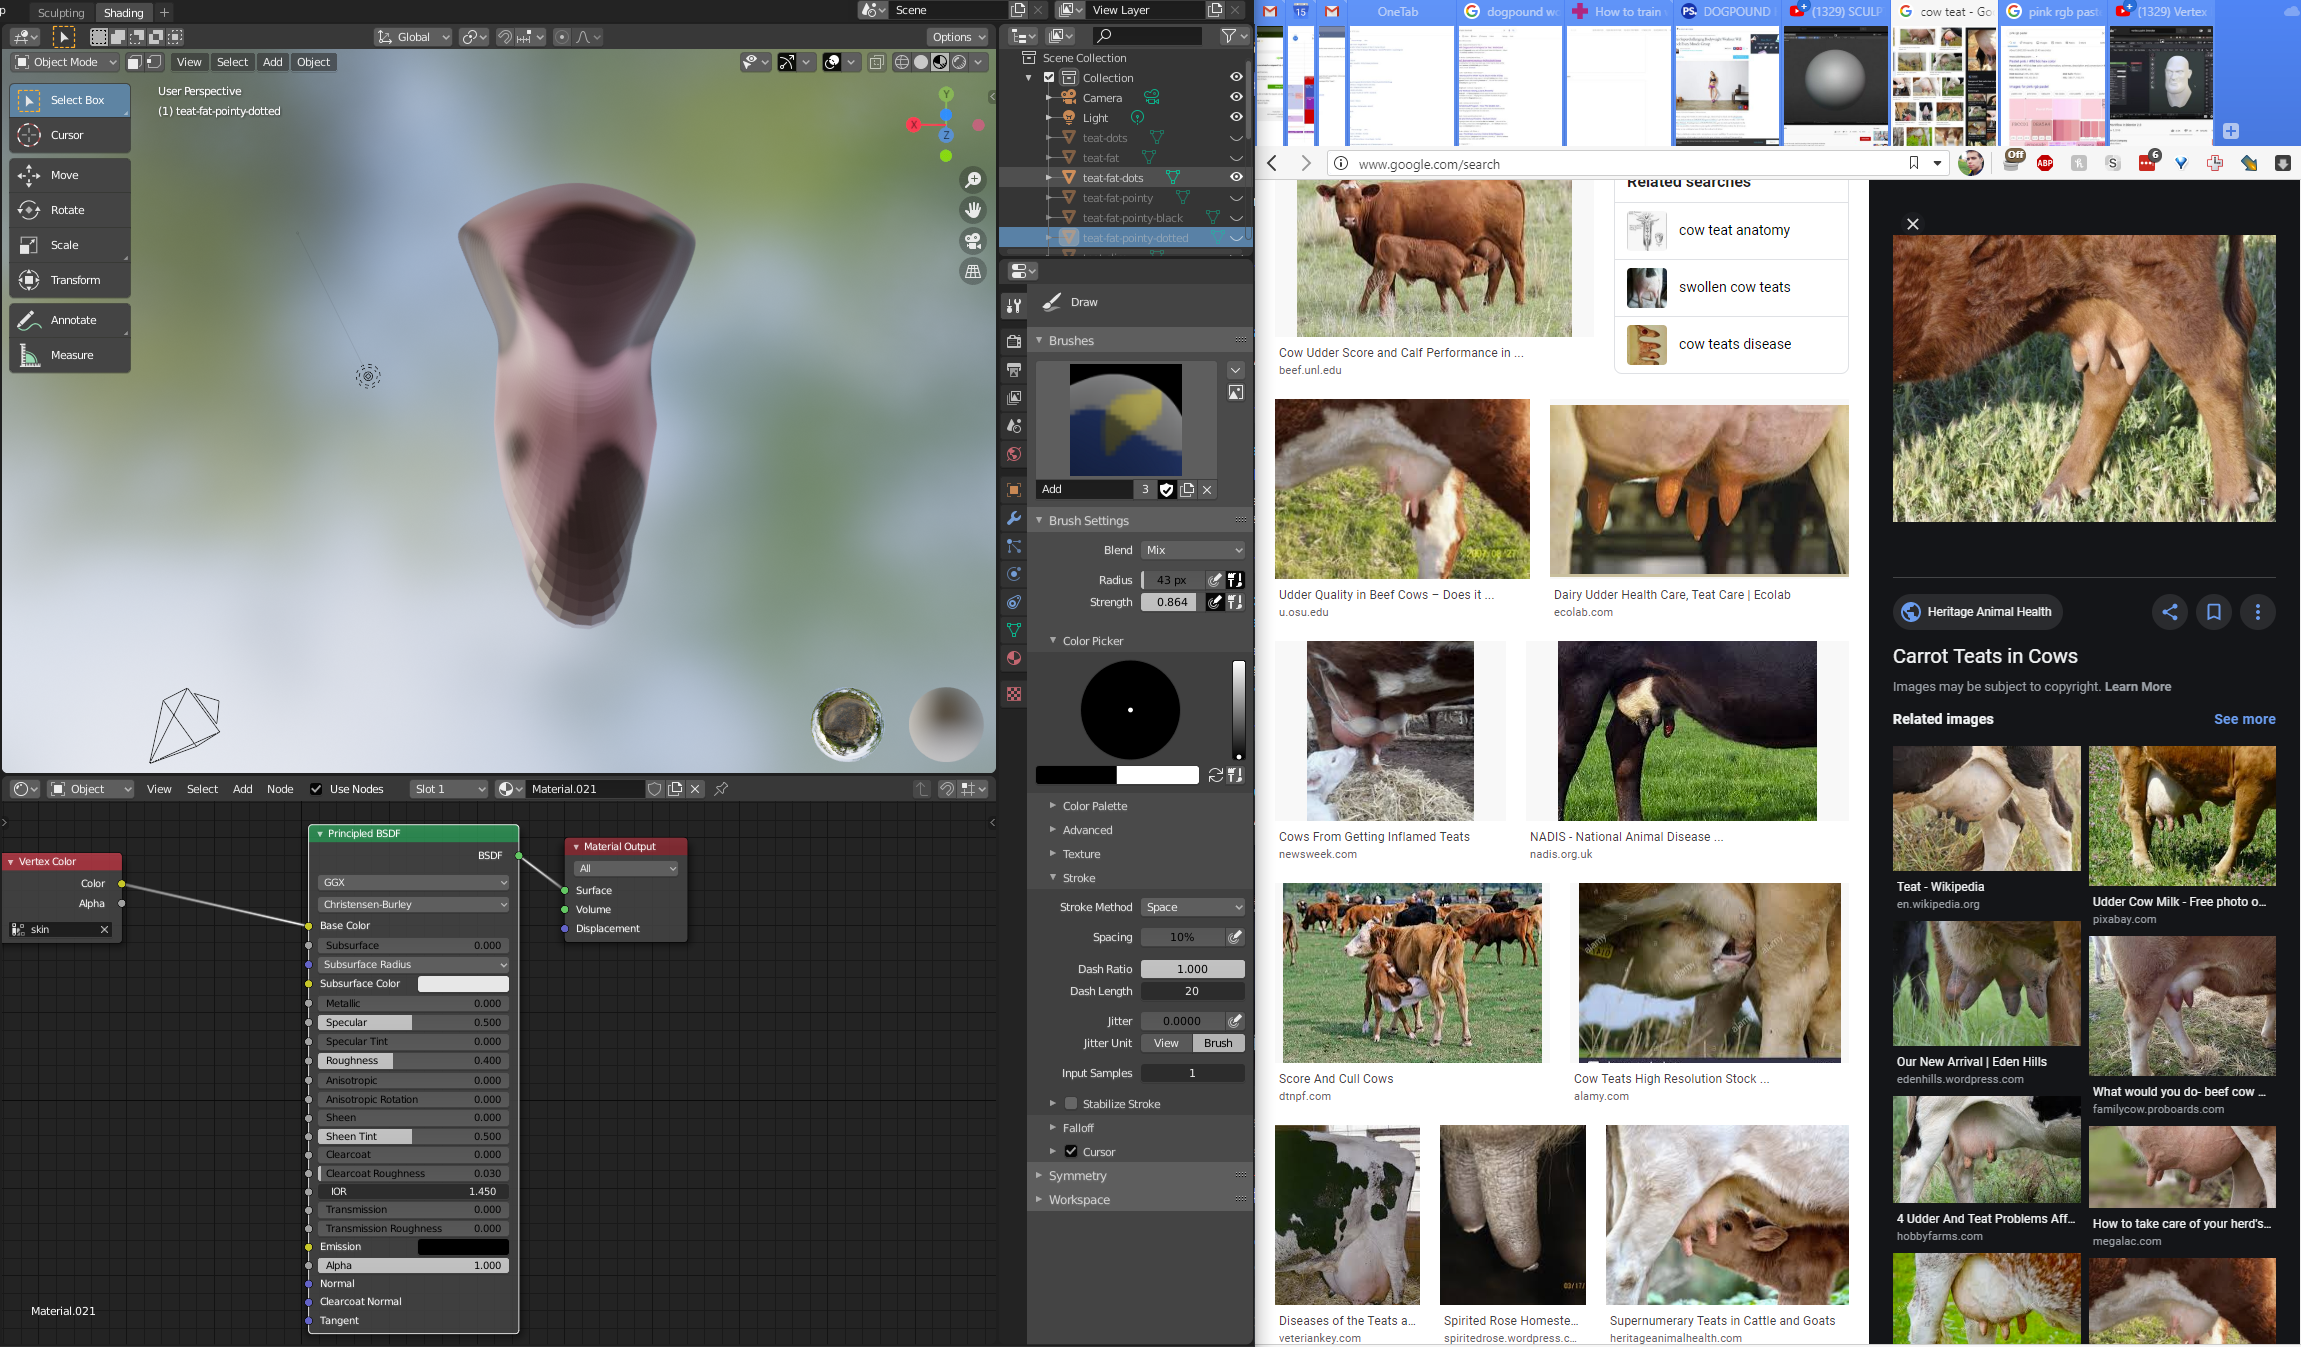
\includegraphics[width=.8\textwidth]{images/ndds1}
    \caption{Screenshot of a photorealistic scene in Unreal Engine 4.}
    \label{fig:ue4-1}
\end{figure}
\begin{figure}[!ht]
    \centering
    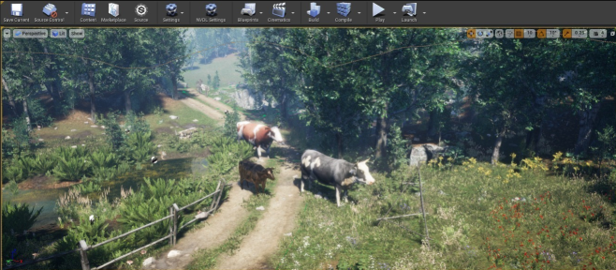
\includegraphics[width=.8\textwidth]{images/ndds2}
    \caption{Screenshot of a photorealistic scene in Unreal Engine 4.}
    \label{fig:ue4-2}
\end{figure}
\begin{figure}[!ht]
    \centering
    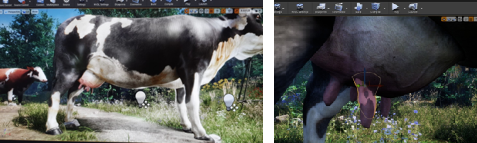
\includegraphics[width=0.8\textwidth]{images/ndds3}
    \caption{Screenshot of a photorealistic scene in Unreal Engine 4.}
    \label{fig:ue4-3}
\end{figure}
% \begin{figure}[!ht]
%     \centering
%     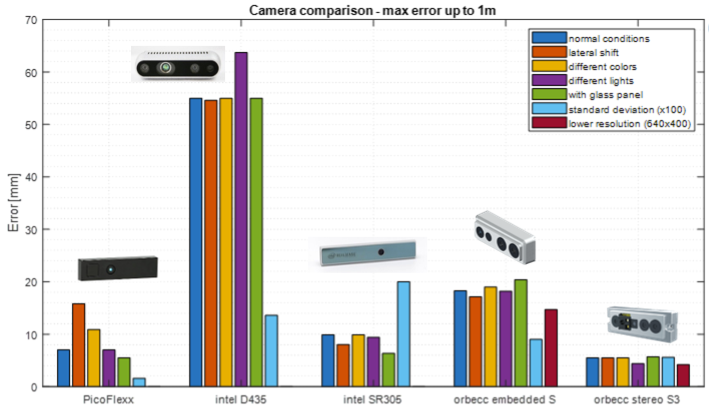
\includegraphics[width=1\textwidth]{images/camera_choice.png}
%     \caption{Screenshot of a sample export from the NDDS plugin.}
%     \label{fig:ndds}
% \end{figure}

\newpage
\section{Pose Estimation Processing Pipeline}
\label{appendix:cow_design}
\begin{figure}[!ht]
    \centering
    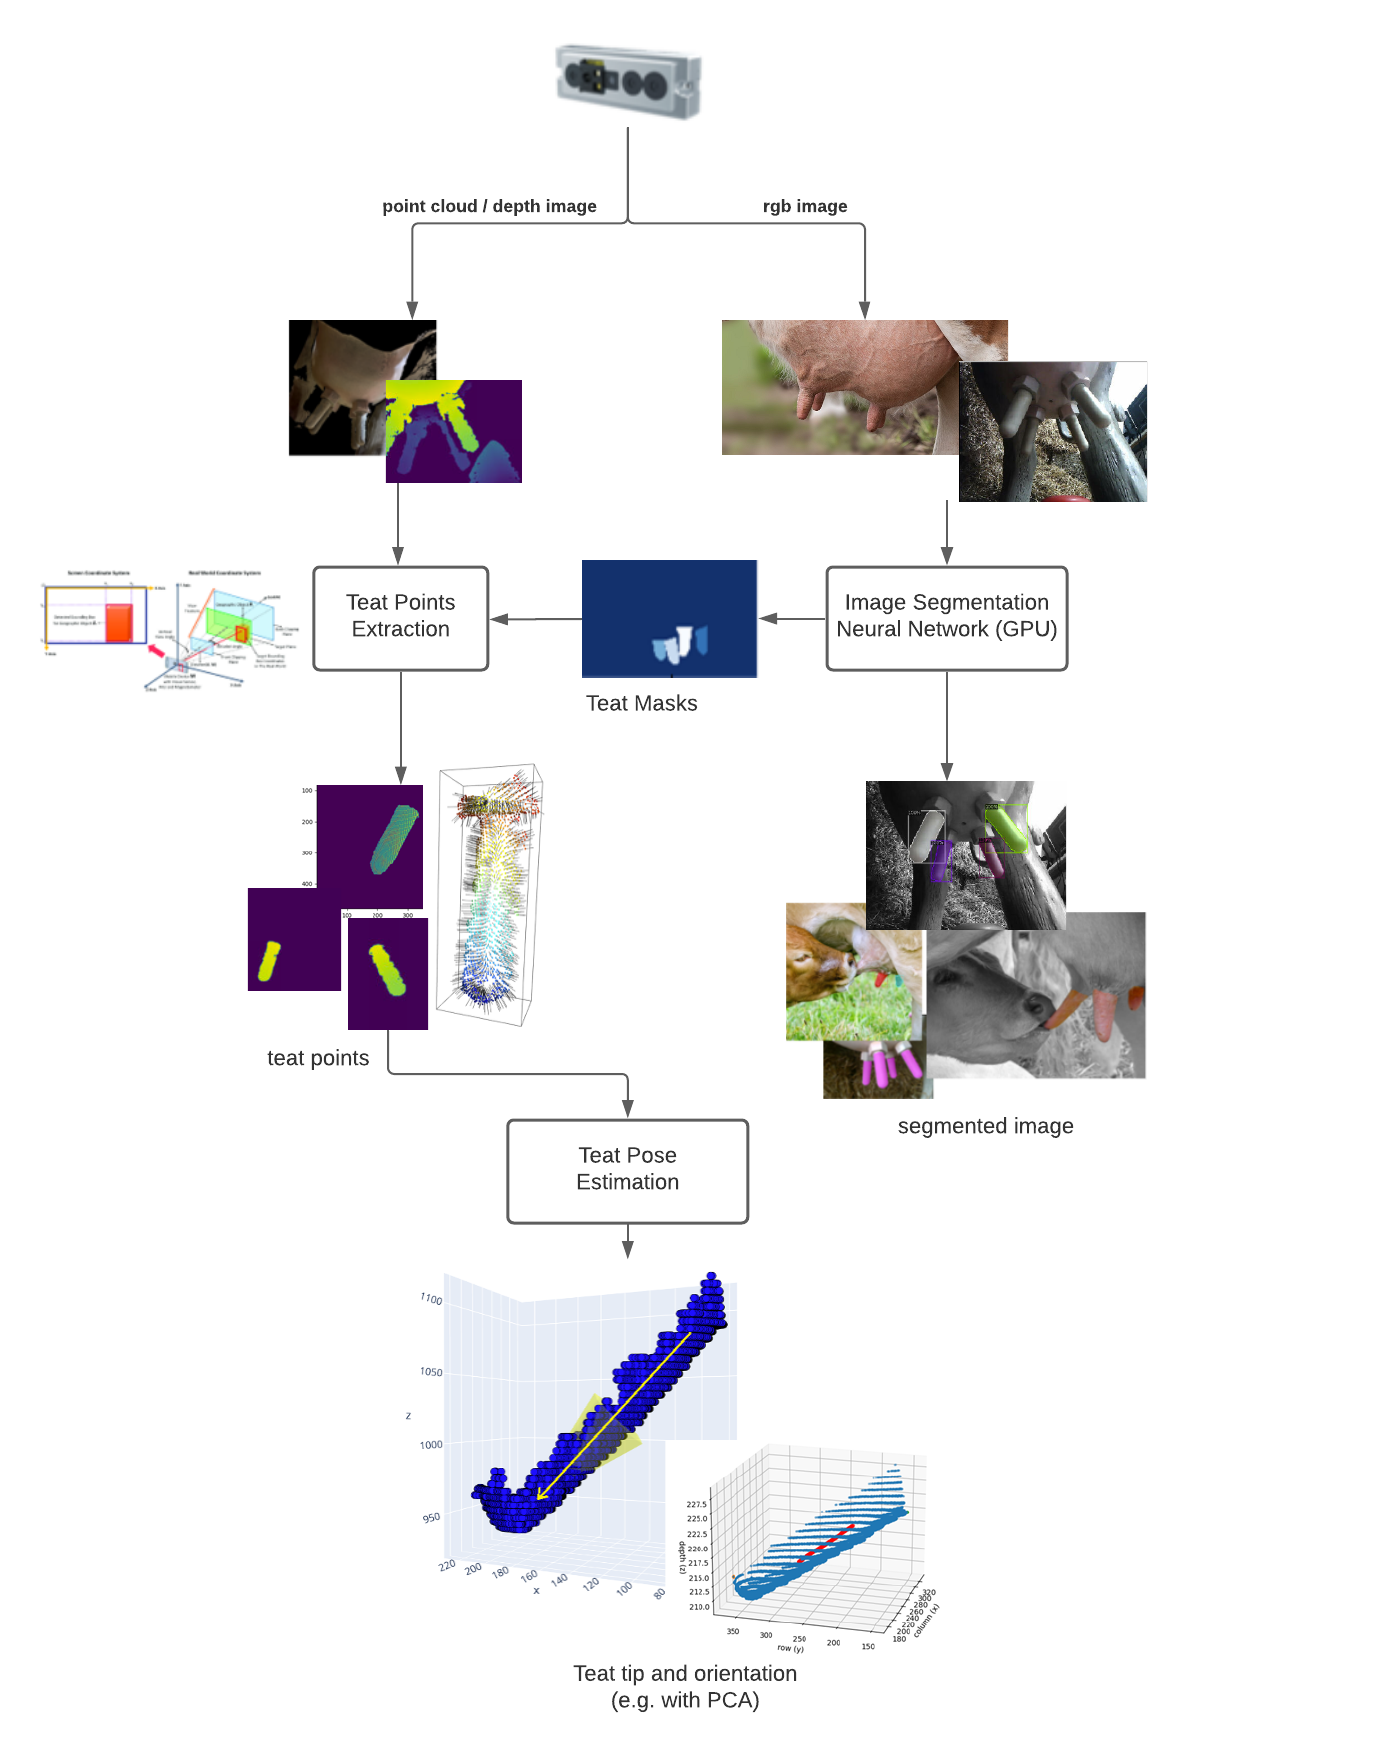
\includegraphics[width=1\textwidth]{images/cow_design.png}
    \caption{Pose Estimation Processing Pipeline Flowchart}
    \label{fig:cow_design}
\end{figure}

\newpage
\section{Camera Evaluation}
\label{appendix:camera_evaluation}

\begin{figure}[h]
        \centering
        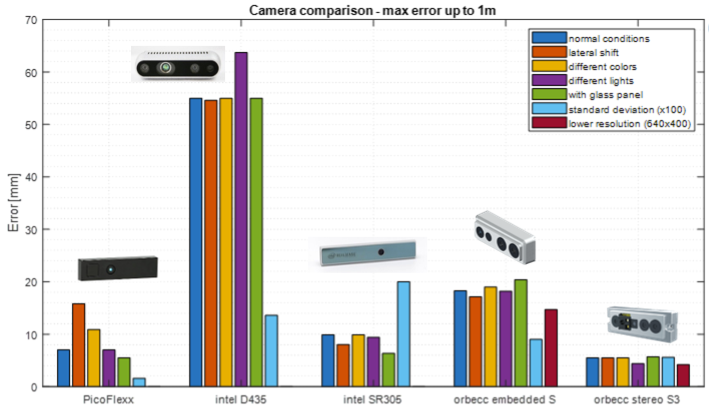
\includegraphics[width=0.8\textwidth]{images/camera_choice.png}
        \caption{Camera Performance Evaluation}
        \label{fig:camera_choice}
    \end{figure}
  
  
  
\newpage
\section{Pose Estimation Error Correlogram}  
\label{appendix:correlogram}
\begin{figure}[h]
        \centering
        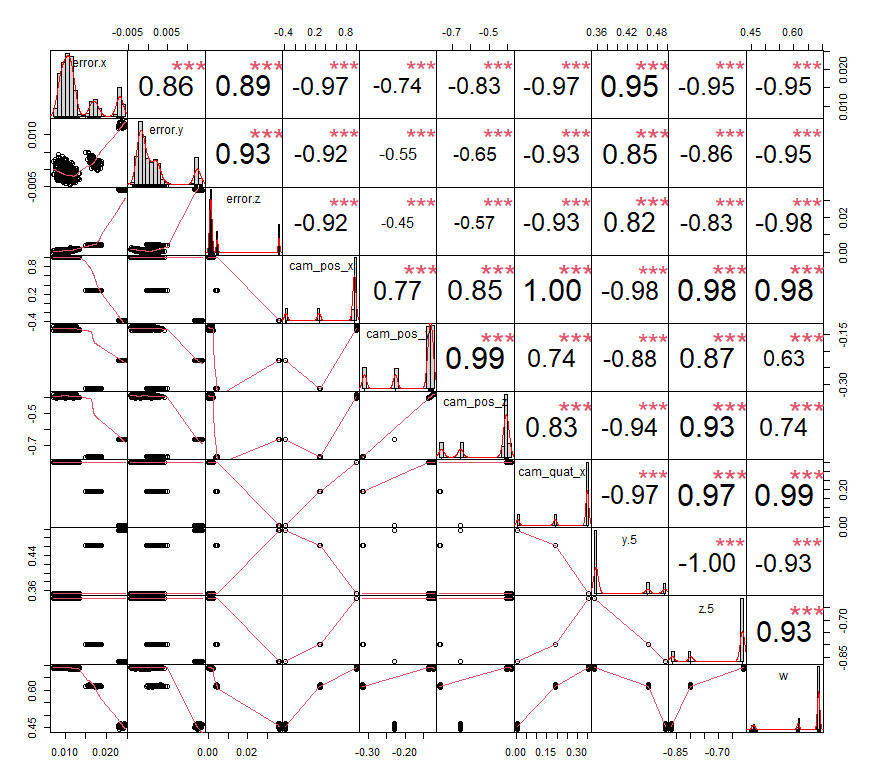
\includegraphics[width=0.9\textwidth]{images/r_correlogram.png}
        \caption{Correlogram of the errors in (x, y, z) and the camera position variables (x, y, z, quaternion) for the MAV algorithm.}
        \label{fig:correlogram}
\end{figure}
